% results.tex (chundawat-h)
% Numbers from notebooks/05_results_analysis.ipynb and results/final_results*.csv,
% layout_gain_bootstrap.csv, bert_vs_layoutlm_wins.csv, error_types.csv.

\section{Results and analysis}
\label{sec:results}

\subsection{Main results}

Table~\ref{tab:main} compares the three methods against the main gold
and Table~\ref{tab:official} against the official answers;
Figure~\ref{fig:f1} shows both.

\begin{table}[t]
  \centering
  \small
  \begin{tabular}{lccccc}
    \toprule
    Field     & Regex & BERT & LayoutLM & Layout gain & 95\% CI of gain \\
    \midrule
    Company   & 68.3 & 89.3 & \textbf{92.9} & $+3.6$ & $[0.9, 6.5]$ \\
    Date      & 95.8 & 97.8 & \textbf{98.7} & $+0.9$ & $[0.0, 2.0]$ \\
    Address   & 59.9 & 91.1 & \textbf{93.7} & $+2.6$ & $[0.9, 4.6]$ \\
    Total     & 75.2 & 89.4 & \textbf{89.5} & $+0.1$ & $[-3.1, 3.6]$ \\
    \midrule
    Macro avg & 74.8 & 91.9 & \textbf{93.7} & $+1.8$ & $[0.5, 3.2]$ \\
    \bottomrule
  \end{tabular}
  \caption{Test $F_1$ (\%) against the main gold (347 receipts). Layout
  gain = LayoutLM $-$ BERT, with its 95\% confidence interval from a
  paired bootstrap over receipts (2{,}000 resamples).}
  \label{tab:main}
\end{table}

\begin{table}[t]
  \centering
  \small
  \begin{tabular}{lcccc}
    \toprule
    Field     & Regex & BERT & LayoutLM & Ceiling \\
    \midrule
    Company   & 57.6 & 72.8 & \textbf{75.2} & 80.4 \\
    Date      & 95.8 & 95.0 & \textbf{96.1} & 96.3 \\
    Address   & 40.9 & 55.6 & \textbf{57.1} & 58.2 \\
    Total     & 77.2 & \textbf{86.5} & 86.0 & 96.3 \\
    \midrule
    Macro avg & 67.9 & 77.5 & \textbf{78.6} & 82.8 \\
    \bottomrule
  \end{tabular}
  \caption{Test $F_1$ (\%) against the official ICDAR answers. Ceiling =
  perfect word tagging (Table~\ref{tab:ceiling}).}
  \label{tab:official}
\end{table}

\begin{figure}[t]
  \centering
  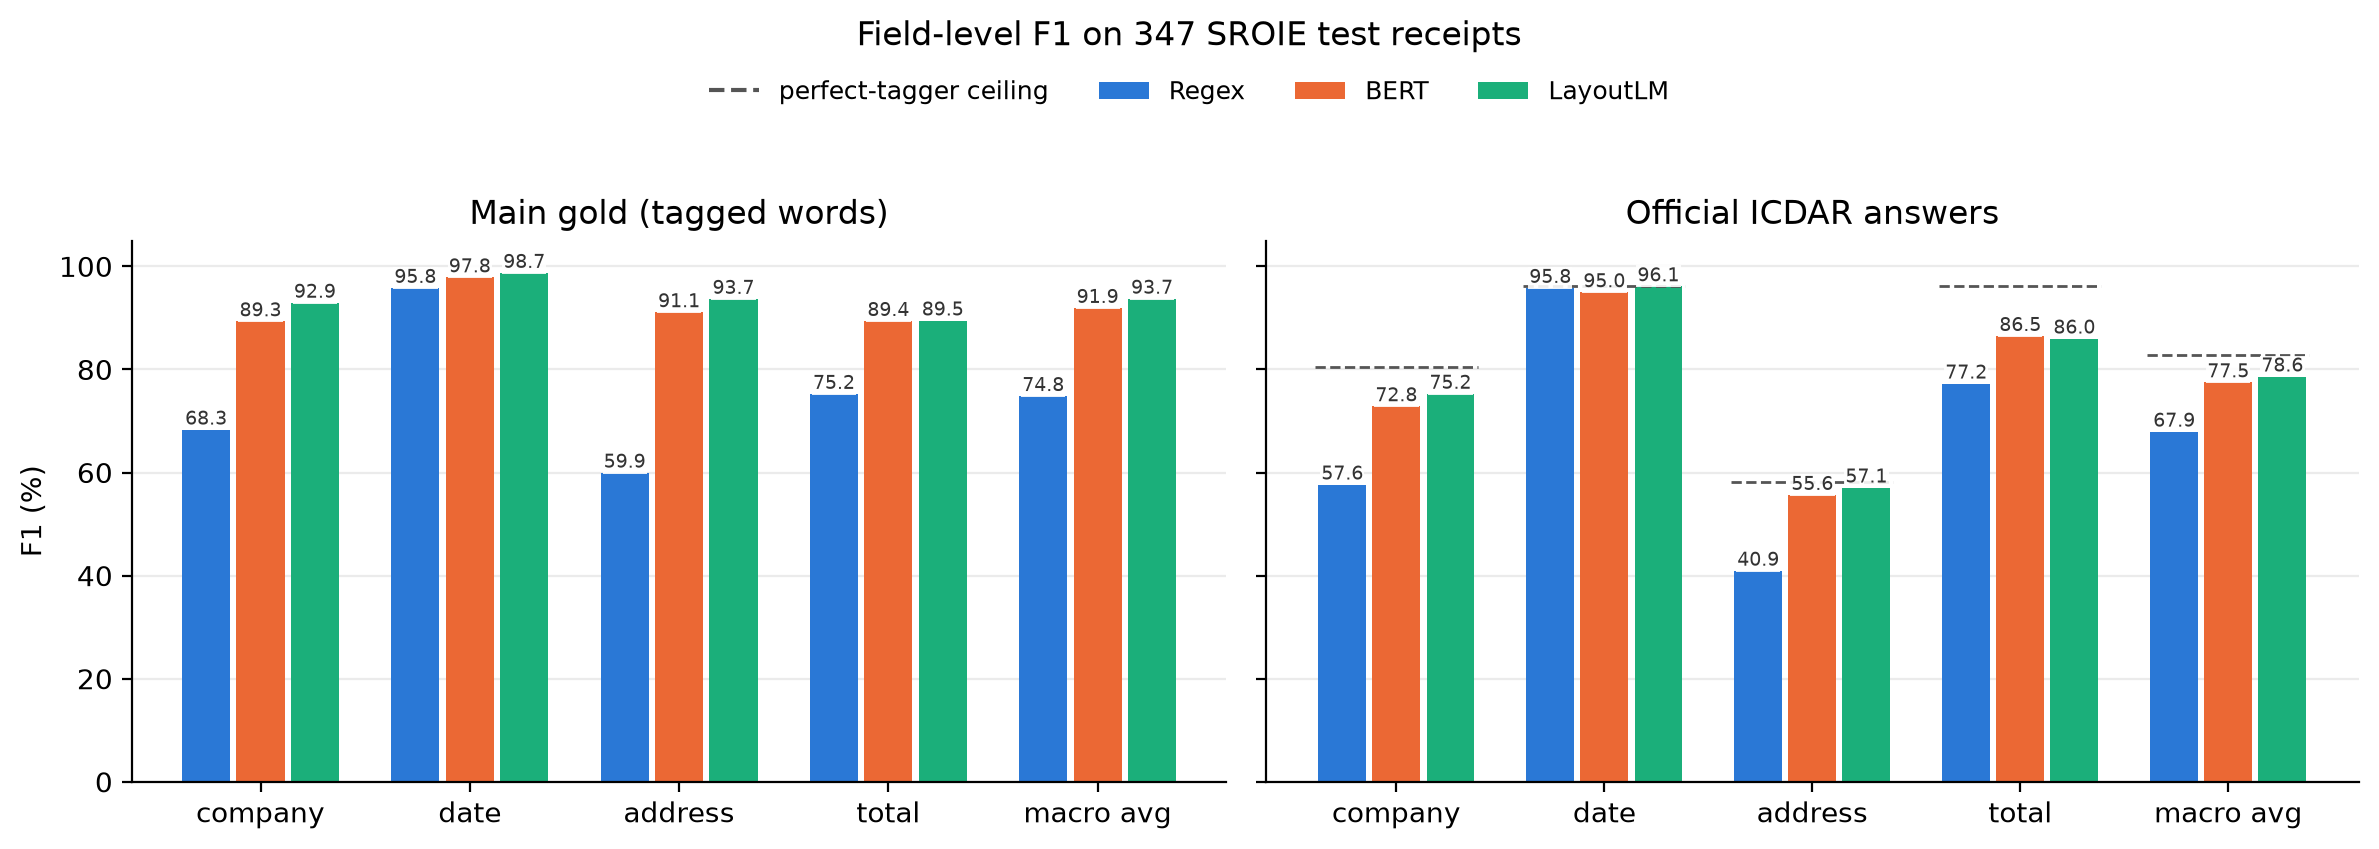
\includegraphics[width=\linewidth]{f1_comparison.png}
  \caption{Per-field test $F_1$ of the three methods against the main
  gold (left) and the official answers (right). Dashed lines mark the
  perfect-tagging ceiling.}
  \label{fig:f1}
\end{figure}

\subsection{Regex baseline}

The baseline reaches 74.8\% macro $F_1$ (76.7\% on the training split it
was tuned on, so it is not over-fitted). Its strengths and failures are
clear-cut:
\begin{itemize}
  \item \textbf{Date} (95.8\%) is almost solved by patterns, because
        dates have a fixed, distinctive format. Most remaining errors are
        label artefacts: some gold date spans include extra words such
        as \texttt{Date:} or a time (Section~\ref{sec:dataset}), which
        the regex correctly leaves out.
  \item \textbf{Total} (75.2\%) fails when a receipt prints several
        totals (before and after rounding, inside GST summary tables) or
        when OCR splits a number.
  \item \textbf{Company} (68.3\%) fails when other text sits above the
        name (\texttt{*** COPY ***}, the cashier's name) or when the name
        has no keyword such as \texttt{SDN BHD}.
  \item \textbf{Address} (59.9\%) is the hardest: its start and end vary,
        and the labels are not consistent about including registration
        numbers or trailing lines.
\end{itemize}

\subsection{Text only vs.\ text + layout}

\paragraph{Learning vs.\ rules.} Text-only BERT improves macro $F_1$ by
17.1 points over the rules ($74.8 \rightarrow 91.9$). The largest gains
are on the free-form fields, address ($+31.1$) and company ($+21.0$),
where rules cannot know where a block starts and ends. Date gains only
2 points because patterns already solve it.

\paragraph{Layout gain.} With the same tokenizer, data and
hyperparameters, adding 2D positions raises macro $F_1$ by a further 1.8
points, to 93.7\%. Because the test set is small, we estimate the
uncertainty with a paired bootstrap: we resample the 347 receipts with
replacement 2{,}000 times and recompute both models' $F_1$ on each
resample. The macro gain is positive in 99.6\% of resamples (95\% CI
$[0.5, 3.2]$). Per field (Table~\ref{tab:main}), the gain is clearly
positive for company ($+3.6$) and address ($+2.6$), borderline for date
($+0.9$) and zero for total ($+0.1$, CI $[-3.1, 3.6]$).
Table~\ref{tab:wins} shows the same picture per receipt: on company and
address, LayoutLM fixes many more receipts than it breaks, while on the
total the two models simply make \emph{different} mistakes (22 vs.\ 23
receipts).

\begin{table}[t]
  \centering
  \small
  \begin{tabular}{lcccc}
    \toprule
     & Company & Date & Address & Total \\
    \midrule
    Only LayoutLM correct & 20 & 4 & 10 & 22 \\
    Only BERT correct     &  8 & 1 &  1 & 23 \\
    Both correct          & 301 & 338 & 315 & 284 \\
    Both wrong            & 18 & 4 & 21 & 18 \\
    \bottomrule
  \end{tabular}
  \caption{Receipt-level agreement of BERT and LayoutLM on the 347 test
  receipts (main gold).}
  \label{tab:wins}
\end{table}

\paragraph{Why layout helps company and address.} Both fields are
\emph{blocks} of one or more lines near the top of the receipt, and
where a block starts and ends is easier to see on the page than in the
word sequence. A text-only model sees the shop name, registration
number, address and mall name as one stream of words. BERT's errors on
these fields are therefore mostly boundary errors: it adds a
neighbouring line or drops the first word (Table~\ref{tab:errors}).
LayoutLM sees the line breaks and the vertical gaps between blocks. It
reduces ``too long'' address predictions from 14 to 6 and ``too short''
company predictions from 12 to 3.

\paragraph{Why layout does not help the total.} One would expect the
total to benefit most, since it sits on the line that says ``TOTAL''.
However, the training labels do not give a consistent position: only
about two thirds of TOTAL tags lie on such a line, and the rest mark
another copy of the amount, such as the item price in
Figure~\ref{fig:receipt} (Section~\ref{sec:dataset}). The model
therefore cannot learn ``take the amount next to TOTAL''. In addition,
field-level exact match is strict: at the word level LayoutLM \emph{is}
better on the total (\texttt{seqeval} span $F_1$ 84.8\% vs.\ 81.5\%),
but a single extra predicted span (e.g.\ \texttt{24.525 26.00}) makes
the whole field wrong, and both models still produce 10--14 such
outputs.

\paragraph{Official answers and OCR noise.} Against the official answers
(Table~\ref{tab:official}) the layout gain shrinks to 1.1 points (95\%
CI $[-0.01, 2.4]$, borderline). LayoutLM is within 1.2 points of the
perfect-tagging ceiling on date and address and about 5 points below it
on company, so most of its remaining errors on these fields come from
OCR, not from tagging. The total is the exception (86.0\% vs.\ a 96.3\%
ceiling), for the labelling reason above. The regex baseline even scores
\emph{higher} on the total against the official answers (77.2\%) than
against the main gold (75.2\%): it reads the amount from the ``TOTAL''
line, while the gold tags often point to another copy of it.

\subsection{Error analysis}

Table~\ref{tab:errors} lists typical receipts on which the two models
disagree.

\begin{table}[t]
  \centering
  \small
  \begin{tabular}{lp{0.36\linewidth}p{0.40\linewidth}}
    \toprule
    Field & Gold & Wrong prediction \\
    \midrule
    \multicolumn{3}{l}{\emph{LayoutLM correct, BERT wrong}} \\
    Company & UROKO JAPANESE CUISINE SDN BHD & JAPANESE CUISINE SDN BHD \\
    Company & GRAND COMPANIONS SON BHD & \textbf{CITY} GRAND COMPANIONS SON BHD \\
    Address & No 8, Jalan 7/118B, Desa Tun Razak 56000 Kuala Lumpur, Malaysia
            & \ldots\ Kuala Lumpur, Malaysia \textbf{CHERAS LEISURE MALL} \\
    Address & 2 \& 2A, Jalan Kasuarina I/KS 7, Bandar Botanik, 41200 Klang, SELANGOR
            & \textbf{001869250560} 2 \& 2A, Jalan Kasuarina \ldots \\
    Date    & 11-01-16 & \textbf{10/2000} 11-01-16 \\
    Total   & 269.40 & \textbf{15.25} 269.40 \\
    \midrule
    \multicolumn{3}{l}{\emph{BERT correct, LayoutLM wrong}} \\
    Company & SIN LIANHAP SON BHD & SIN LIANHAP SON BHD \textbf{SON BHD} \\
    Company & HUGO TRADING SDN BHD & HUGO TRADING SDN BHD \textbf{Tota} \\
    Total   & 6.35 & 6.36 \\
    Total   & 26.00 & \textbf{24.525} 26.00 \\
    \bottomrule
  \end{tabular}
  \caption{Disagreements between BERT and LayoutLM (test set, main gold).
  Bold marks extra words; \texttt{SON BHD} is an OCR error for
  \texttt{SDN BHD} that is also in the gold.}
  \label{tab:errors}
\end{table}

BERT's typical company and address errors are boundary errors: it drops
a leading word (UROKO), absorbs a neighbouring line (CITY, CHERAS
LEISURE MALL) or attaches a registration number. LayoutLM fixes these by
seeing which words share a line or block. Its own errors are fewer but
of the same kind, e.g.\ tagging the repeated \texttt{SON BHD} on the
next line or a stray word (\texttt{Tota}) below the name. On the total,
both models mainly fail by choosing the wrong copy of an amount or by
tagging two amounts. Since the labels themselves are not consistent
about which copy is the total, layout cannot fix this.
